\chapter{List of evaluated tools}
\label{chapter:first-appendixa}
\begin{figure}[!ht]
    \begin{center}
      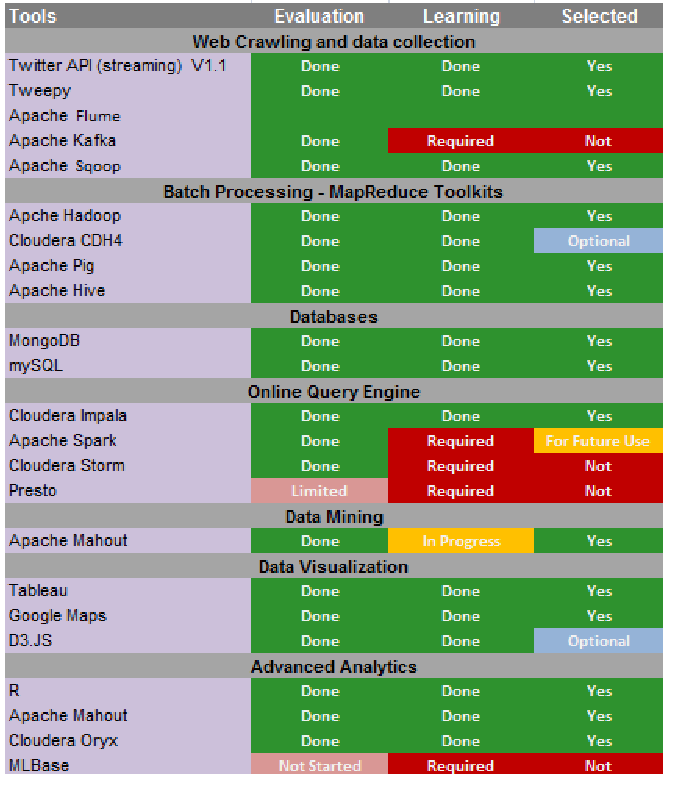
\includegraphics[scale=0.92]{images/appenda.pdf}
      \caption{List of evaluated platform components.}
      \label{fig:list_eval}
    \end{center}
\end{figure} 

\chapter{Data Descriptions}
\label{chapter:appendixc}

\section{Hourly consumption data}

Contains the hourly utility consumption data recorded by the specialized meters, installed by VTT in test buildings as Green Campus initiative test sites. These devices measures consumption of following utility types.
\begin{enumerate}

\item S{\"A}KH{\"O} (Electricity);( consumption /100) will be KWh values
\item KAUKOL{\"A}MP{\"O}(District Heating-);same unit as above
\item LOISTEHO (Reactive-Power) -KVar
\item VESI(water) in \(m^3\)
\item Data header is not available in data, please follow the description.
\end{enumerate}
There are 8 comma separated fields in the each record / row. Description is as the following, 
\begin{enumerate}
\item Device ID: are the unique codes to identify the metering device installed in buildings. One building may have more than one device.
\item Building Names in Finnish language. You may require the appropriate encoding e.g utf-8 to read the names
\item Building Address in Finnish language. You may require the appropriate encoding e.g utf-8 to read the addresses.
\item Meter Type is related to utility type value 1 to 4
\item Utility type. Four types explained above. Text in Finnish language. You may require the appropriate encoding e.g utf-8 to read the names
\item Date YYYYMMDD of collected record
\item Hour of the day, Value from 0 to 23. 0 hour mean utility consumed from 00:00 to 00:59 hr of the day.
\item Consumption value of utility. Units as explained above.
\end{enumerate}

\section{NIALM Device Data}
This data is collected from the NIALM device installed in one of the test site- a residential student-family apartment.
\begin{enumerate}
\item First row describes the time zone setting.
\item Second row is the header.
\item Data fields are separated by ;
\item Each record contains the name of the device used, time stamp of usage and the amount of electricity consumed in Watt hour unit.
\item Please note that there are certain devices that are being logged into records after their respective usage however there are devices like refrigerator and freezer that are being used continuously and NIALM device uses internal mechanism to get consumption value of these devices after certain period of time.
\end{enumerate}

 

\chapter{Detailed Results}
\label{chapter:appendixd}
\section{K-means clustering}
\begin{figure}[!ht]
    \begin{center}
      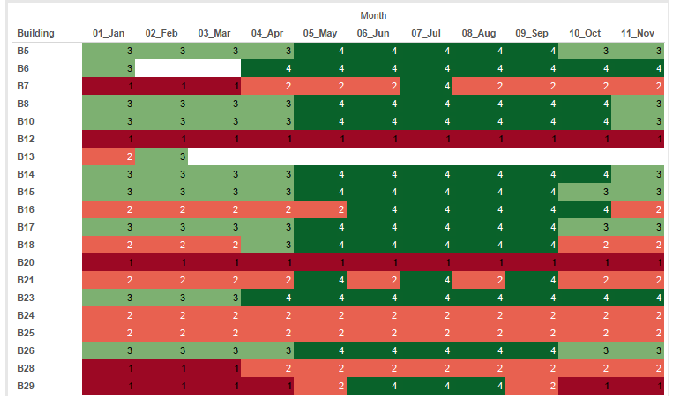
\includegraphics[width=\textwidth]{images/appendd1.pdf}
      \caption{Details of K-means clustering results. Four classes of buildings are represented as high efficiency (4), moderate efficiency (3), low efficiency (2), and poor efficiency (1).}
      \label{fig:kmeans_detail}
    \end{center}
\end{figure} 



\newgeometry{left=2.0cm,bottom=0.1cm}
\section{Base loads}
\begin{table}[!ht]
\begin{tabular}{ | l | l | l | l | l | l | l | l | l | l | l | l | }
\hline
	Building & Jan & Feb & Mar & Apr & May & Jun & Jul & Aug & Sep & Oct & Nov \\ \hline
	Building 12 & 406.2 & 410.5 & 414.5 & 395.9 & 399 & 426.3 & 422.2 & 431.2 & 417.2 & 419.9 & 431.2 \\ \hline
	Building 24 & 289.3 & 292.3 & 289.3 & 291.8 & 306.1 & 313.2 & 310.5 & 316.8 & 321.7 & 322.1 & 319.3 \\ \hline
	Building 2 & 251.7 & 254.1 & 255.3 & 257.39 & 255.5 & 279.7 & 271.8 & 275.3 & 268.1 & 256.1 & 245.3 \\ \hline
	Building 20 & 227.9 & 235.8 & 234.4 & 239.5 & 247.7 & 259.1 & 255.9 & 265.6 & 268.3 & 258.1 & 244.9 \\ \hline
	Building 31 & 170.3 & 175.7 & 163.1 & 159.6 & 182.8 & 195.4 & 190.4 & 176 & 177.9 & 164.6 & 164.7 \\ \hline
	Building 14 & 78.2 & 57.1 & 54.4 & 50.4 & 52.2 & 49.4 & 45.3 & 46.9 & 50.9 & 52.4 & 56.1 \\ \hline
	Building 11 & 77.8 & 83.7 & 83.7 & 83.4 & 74 & 66.5 & 59.7 & 55.2 & 51.7 & 72.5 & 75 \\ \hline
	Building 28 & 62.3 & 66.8 & 68 & 71.9 & 73.2 & 73.90 & 67.7 & 67.5 & 68.5 & 65.7 & 69.2 \\ \hline
	Building 8 & 60.9 & 65 & 63.3 & 68 & 72.3 & 75.7 & 75.59 & 73.5 & 67.5 & 68 & 65.5 \\ \hline
	Building 25 & 60.3 & 61.4 & 61.7 & 60.6 & 71.2 & 69.59 & 60.6 & 62.1 & 51.4 & 50 & 45.5 \\ \hline
	Building 10 & 59.3 & 54 & 53 & 45.2 & 50.8 & 53.9 & 56.5 & 55.9 & 57.6 & 59 & 57.5 \\ \hline
	Building 6 & 56.2 & 0 & 0 & 183.9 & 231.7 & 239.9 & 232.8 & 228.6 & 400.2 & 223.6 & 205.3 \\ \hline
	Building 17 & 48 & 48.1 & 47 & 44.2 & 45 & 46.3 & 44.8 & 48.2 & 48.6 & 48.6 & 47.4 \\ \hline
	Building 26 & 44.3 & 44.7 & 44.7 & 56.1 & 59.1 & 63.1 & 59.8 & 59.9 & 60.9 & 56.3 & 49.5 \\ \hline
	Building 5 & 43.6 & 45.8 & 45.6 & 44.6 & 46.8 & 50.9 & 50.5 & 52.7 & 85.4 & 47.1 & 47.6 \\ \hline
	Building 21 & 41.9 & 45.8 & 42.4 & 38.5 & 39.2 & 47.2 & 42.7 & 46.5 & 40.5 & 40.2 & 40.4 \\ \hline
	Building 16 & 38.5 & 43.3 & 42.2 & 40.2 & 40.7 & 41.2 & 36.1 & 41.9 & 33.9 & 31.8 & 35.7 \\ \hline
	Building 22 & 31.1 & 27.8 & 32 & 36.1 & 37 & 34.9 & 32.7 & 33.6 & 35.5 & 36.4 & 39.1 \\ \hline
	Building 7 & 30.9 & 42.1 & 44.1 & 41.7 & 38 & 37.2 & 26.1 & 39.5 & 35.4 & 44.4 & 43.3 \\ \hline
	Building 1 & 25.2 & 26.2 & 23.4 & 21.6 & 22.7 & 24.7 & 22.2 & 24.6 & 23.1 & 22.8 & 29.4 \\ \hline
	Building 23 & 19.8 & 20.3 & 21.2 & 23.1 & 20.6 & 18.8 & 18.7 & 20.5 & 23.9 & 23.7 & 22.7 \\ \hline
	Building 29 & 16.6 & 14.7 & 13.6 & 12 & 10 & 8.6 & 10.7 & 9.6 & 10.4 & 10.9 & 12.7 \\ \hline
	Building 30 & 14.7 & 14.6 & 13.8 & 14.3 & 14.2 & 14 & 13.3 & 13.9 & 13.5 & 11.7 & 11.9 \\ \hline
	Building 18 & 12.5 & 13.2 & 12.8 & 13 & 13.1 & 11.9 & 12.7 & 13.5 & 13.1 & 13.1 & 13.4 \\ \hline
	Building 15 & 9.2 & 10.2 & 10.4 & 10 & 12.6 & 15.8 & 16.6 & 16.2 & 13.2 & 10.4 & 9.8 \\ \hline
	Building 19 & 4.5 & 5.3 & 5.5 & 4.8 & 4.4 & 3.6 & 4.0 & 4.5 & 4.5 & 4.8 & 4.9 \\ \hline
\end{tabular}
\caption{Base loads of the buildings in KWh.}
\end{table}
